\documentclass[sigconf]{acmart}

\usepackage{algorithmic}
\usepackage{algorithm}
\usepackage{hyperref}
\usepackage{listings}

\begin{document}

\title{Lab 7 Exercise - Transforming Sequences}
\author{Luke McClure}
\email{29573904}

\maketitle
\pagestyle{myheadings}

\section{Sequence-to-Sequence Modelling}

The source text must first be passed through the embedding layer that maps a word into a dense vector that the LSTM is able to use.

As the decoder only requires the hidden and cell state of the previous timestep, we can disregard the LSTM output that includes all previous timesteps.
By splitting the hidden state tuple into the hidden state and cell state it is easier to pass back for use by the decoder network.

\begin{lstlisting}[language=Python]
def forward(self, src):
    embedded = self.embedding(src)      
    _, (h, c) = self.rnn(embedded)
        
    return h, c
\end{lstlisting}

The model shows a very clean training curve in \autoref{fig:traincurve}, with the test and training loss closely following each other.

\begin{figure}[h]
	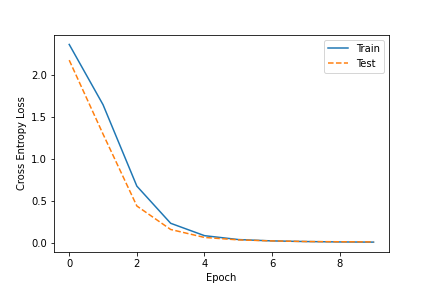
\includegraphics[width=\linewidth]{../traincurve.png}
	\caption{Training curve of seq2seq model}
	\label{fig:traincurve}
\end{figure}	
\subsection{Complete and train a seq2seq model}
\subsection{now use it!}
\label{scn:1.2}
\subsubsection{Why is the order of the output reversed?}\\

The output is reversed as the model is trained to predict the output in reverse. 
Due to the difficulty LSTM's have in learning long range dependancies, reversing the output means that the end characters of the input sequence will be beside the corresponding correctors in the target sequence. This shortens the dependencies the LSTM needs to learn at first in order to build up the translation model. 
\subsubsection{What is the point of teacher forcing?}\\

During normal output the RNN would use the previous character to predict the character at timestep t, so if the model were to predict the character incorrectly this would carry through for the rest of the sentence.
Teacher forcing provides the model with the correct output before prediction of the next character during training. 
This means that instead of trying to build off an incorrect prediction the model is given another opportunity to correctly learn, speeding up backpropogation and therefore speed up convergence.
\subsection{Sequence lengths}
The first string in \autoref{scn:1.2} was chunked to factors of it's original length, these factors were 1, 3, 23 \& 69.
\begin{itemize}
    \item [1] et te eee ett e ete   t eeee e   eete ttt etee etee ttt ett ee te tte
    \item [3] t amen\^mst a tet aee e t\^mseeeet \^oumett m\^oreee\^edt m tet m iemen\^ng
    \item [23] \^\^\^\^\^\^\^\^\^\^\^\^\^\^\^ gavert \^\^\^\^\^\^\^\^\^\^\^\^\^\^\^\^\^ he fol\^\^\^\^\^\^\^\^\^\^\^\^\^\^\^\^\^ lowing
    \item [69] \^\^\^\^\^\^\^\^\^\^\^\^\^\^\^\^\^\^\^\^\^\^\^\^\^\^\^\^\^\^\^\^\^\^\^\^\^\^\^\^\^\^\^\^\^\^\^\^\^\^\^\^\^\^\^\^\^\^ e lovelwing
\end{itemize}
The model starts to break down with longer chunks. While single letters only produces outputs consisting of the most common letters in the English language, chunks of half or the length of the sentence start to only get predicted as the starting character.
With a mean input length of 12.4 and target length of 3.5 this is not too surprising, the training data consists of several character slices long of text so chunks closely matching that training size will perform better.
\end{document}
\endinput